\documentclass{article}
\usepackage{graphicx}
\graphicspath{{figures/}}
\title{Varlens: annotating a personal genome on your own computer}
\begin{document}
\maketitle

\section{Introduction}
People who receive their genome as a variant file cannot read it. Varlens reads it locally.
% Figure~\ref{fig:old} was the screenshot we dropped.

\section{Results}
Varlens annotated the genome in a median of 31.4~s (Figure~\ref{fig:runtime}).

\begin{figure}
  \centering
  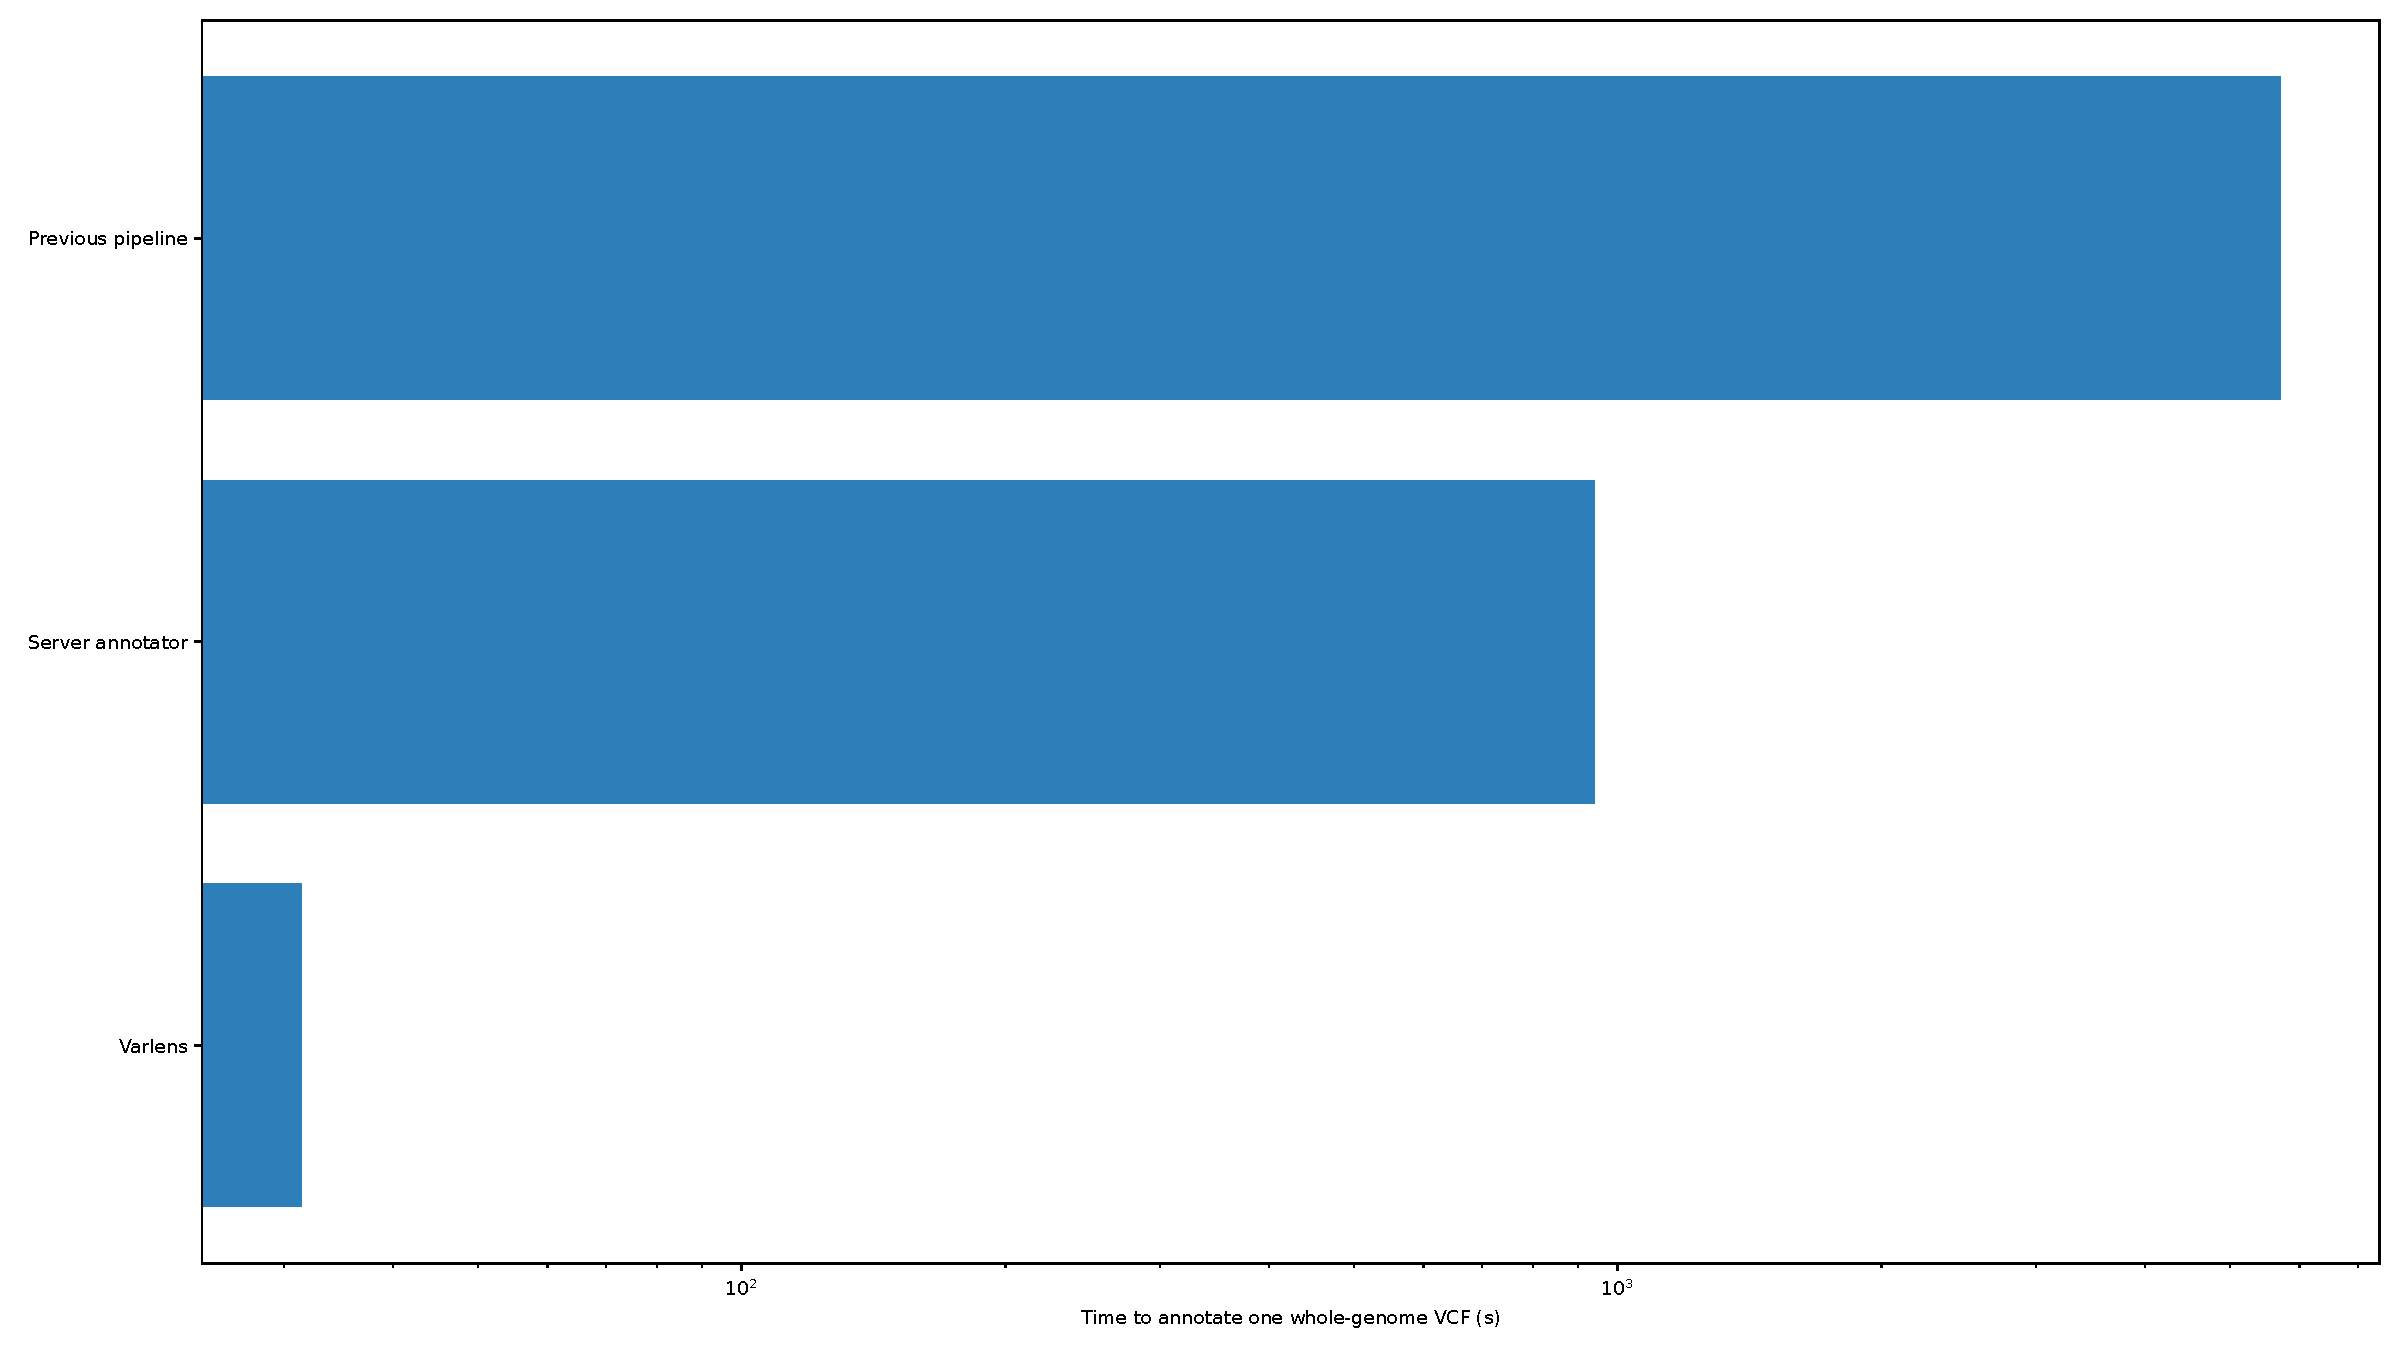
\includegraphics[width=\columnwidth]{runtime}
  \caption{Time to annotate one whole-genome VCF: the median of five runs.}
  \label{fig:runtime}
\end{figure}

\begin{figure*}
  \centering
  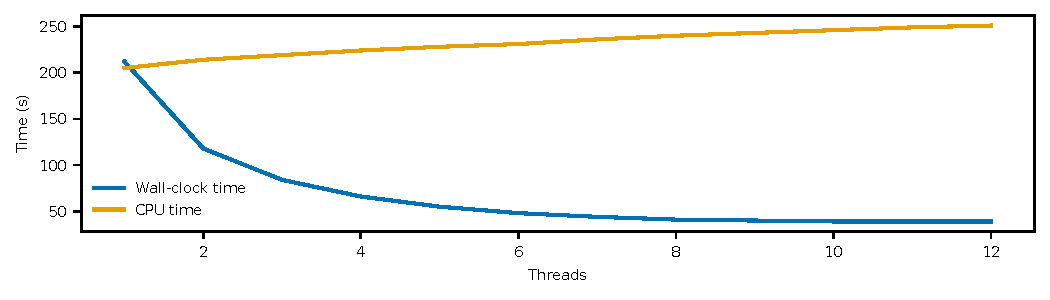
\includegraphics[width=\textwidth]{threads}
  \caption{Wall-clock and CPU time for thread pools of 1 to 12 threads.}
  \label{fig:threads}
\end{figure*}

\begin{figure}
  \centering
  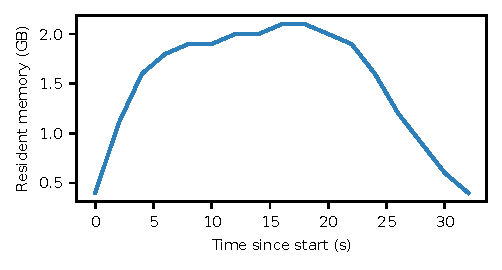
\includegraphics[width=\columnwidth]{memory.pdf}
  \caption{Resident memory during one run.}
  \label{fig:memory}
\end{figure}


\section{Discussion}
Varlens reports associations, not diagnoses; peak memory is in Figure~\ref{fig:peak}.

\end{document}
